\documentclass[xcolor=dvipsnames]{beamer}

\usetheme{Boadilla}

\newcommand{\bi}{\begin{itemize}}
\newcommand{\ei}{\end{itemize}}
\newcommand{\be}{\begin{enumerate}}
\newcommand{\ee}{\end{enumerate}}
\newcommand{\bc}{\begin{center}}
\newcommand{\ec}{\end{center}}
\newcommand{\bd}{\begin{description}}
\newcommand{\ed}{\end{description}}
\newcommand{\I}{\item}
\newcommand{\f}{\frame}
\newcommand{\ft}{\frametitle}
\newcommand{\bcol}{\begin{column}}
\newcommand{\ecol}{\end{column}}
\newcommand{\bcols}{\begin{columns}}
\newcommand{\ecols}{\end{columns}}

\title{HDDM and Track Fitting}
\author[M.\ Ito]{Mark M.\ Ito}
\date{December 3, 2008}
\institute[JLab]{Hall D Software Meeting}

\begin{document}

\frame{\titlepage}

\f{
\centerline{\Large What is XML?}
}
\f{
  \ft{A standard style for ascii-based markup languages}
    \bi
    \I Elements
    \I Attributes
    \I Text
    \I Hierarchical
    \I Example 1: XHTML
    \I Example 2: Menu
    \I Example 3: Powerpoint, Office 2007 (< 1\% of one of 41 slides)
    \ei
}

\begin{frame}[fragile]
\frametitle{Example 2: Menu}
\tiny
\begin{verbatim}
<?xml version="1.0" encoding="ISO-8859-1"?>
<breakfast_menu>
  <food>
    <name>Belgian Waffles</name>
    <price>$5.95</price>
    <description>two of our famous Belgian Waffles with plenty of real maple syrup</description>
    <calories>650</calories>
  </food>
  <food>
    <name>French Toast</name>
    <price>$4.50</price>
    <description>thick slices made from our homemade sourdough bread</description>
    <calories>600</calories>
  </food>
  <food>
    <name>Homestyle Breakfast</name>
    <price>$6.95</price>
    <description>two eggs, bacon or sausage, toast, and our ever-popular hash browns</description>
    <calories>950</calories>
  </food>
</breakfast_menu>
\end{verbatim}
\end{frame}

\begin{frame}[fragile]
\frametitle{Example 3: Powerpoint}
\tiny
\begin{verbatim}
<?xml version="1.0" encoding="UTF-8" standalone="yes"?>
<p:sld xmlns:a="http://schemas.openxmlformats.org/drawingml/2006/main"
  xmlns:r="http://schemas.openxmlformats.org/officeDocument/2006/relationships"
  xmlns:p="http://schemas.openxmlformats.org/presentationml/2006/main">
.
.
.
<a:r>
  <a:rPr kumimoji="0" lang="en-US" sz="1400" b="1" i="0" u="none"
         strike="noStrike" cap="none" normalizeH="0" baseline="0" dirty="0"
         smtClean="0">
    <a:ln>
      <a:noFill/>
    </a:ln>
    <a:solidFill>
      <a:schemeClr val="tx1"/>
    </a:solidFill>
    <a:effectLst/>
    <a:latin typeface="Arial" charset="0"/>
    <a:cs typeface="Arial" charset="0"/>
  </a:rPr>
  <a:t>Service Building Program Power Requirements</a:t>
</a:r>
.
.
.
</p:sld>
\end{verbatim}
\end{frame}

\f{
\ft{Pros and Cons}
  \bi
  \I Advantages
    \bi
    \I Human-readable
    \I Self-documenting
    \I Ubiquitous
      \bi
      \I Lots of books and tutorials
      \I Standard tools: perl, python, java, C, C++,...
      \I Understood by browsers
      \I Here to stay
      \ei
    \ei
  \I Disadvantages
    \bi
    \I A lot of redundant information
      \bi
      \I Not suitable for apps with large data volume
      \ei
    \I Data-centric model
      \bi
      \I Not suitable for object serialization
      \ei
    \ei
  \ei
}

\f{
\centerline{\Large What is HDDM?}
}

\f{
\ft{Lots of Meanings for HDDM}
  \be
  \I A description of an XML language (itself written in XML): a template
    \bi
    \I for Hall D we want a description of an XML language for expressing event data (event.xml)
    \I but the system can describe anything (e. g. a menu)
    \ei
  \I A prescription for compressing the XML data*
    \bi
    \I the template is always written to the data file
      \bi
      \I HDDM data file = template + binary data
      \I preserves self-documenting feature of XML
      \ei
    \I lose human-readability
    \I provides instructions on how to uncompress the data
    \ei
  \I A set of tools (binaries and scripts) for manipulating the data
    \bi
    \I hddm-xml
    \I xml-hddm
    \I hddm-schema*
    \I etc.
    \ei
  \I An auto-generated API for reading and writing data files (from C)*
  \ee
}

\f{
\centerline{\Large What is the format of HDGEANT output?}
}

\begin{frame}[fragile]
\frametitle{HDGEANT template: event.xml}
\tiny
\begin{verbatim}
<?xml version="1.0" encoding="iso-8859-1" standalone="no" ?>
<HDDM xmlns="http://www.gluex.org/hddm" class="s" version="1.0">

  <physicsEvent eventNo="int" maxOccurs="unbounded" runNo="int">
    <reaction maxOccurs="unbounded" minOccurs="0" type="int" weight="float">
      <beam minOccurs="0" type="Particle_t">
        <momentum E="float" px="float" py="float" pz="float"/>
        <properties charge="int" mass="float"/>
      </beam>
      <target minOccurs="0" type="Particle_t">
        <momentum E="float" px="float" py="float" pz="float"/>
        <properties charge="int" mass="float"/>
      </target>
      <vertex maxOccurs="unbounded">
        <product decayVertex="int" id="int" maxOccurs="unbounded" mech="int" parentid="int" pdgtype="int" type="Particle_t">
          <momentum E="float" px="float" py="float" pz="float"/>
          <properties charge="int" mass="float"/>
        </product>
        <origin t="float" vx="float" vy="float" vz="float"/>
      </vertex>
    </reaction>
...
\end{verbatim}
\end{frame}

\begin{frame}[fragile]
\frametitle{HDGEANT data: hdgeant.hddm (output of hddm-xml)}
\tiny
\begin{verbatim}
<?xml version="1.0" encoding="UTF-8"?>
<HDDM class="s" version="1.0" xmlns="http://www.gluex.org/hddm">
  <physicsEvent eventNo="1" runNo="9999">
    <reaction type="0" weight="0">
      <vertex>
        <product decayVertex="0" id="1" mech="0" parentid="0" pdgtype="0" type="pi+">
          <momentum E="0" px="0.042426" py="0.587667" pz="0.860819" />
        </product>
        <origin t="0" vx="0" vy="0" vz="65" />
      </vertex>
    </reaction>
    <hitView version="2.0">
      <centralDC>
        <cdcStraw ring="1" straw="12">
          <cdcStrawHit dE="1.14576e-05" t="116.157" />
        </cdcStraw>
        <cdcStraw ring="2" straw="13">
          <cdcStrawHit dE="3.44262e-06" t="31.0793" />
        </cdcStraw>
...
\end{verbatim}
\end{frame}

\begin{frame}[fragile]
\frametitle{HDGEANT API: C structures}
\tiny
\begin{verbatim}
typedef struct {
   int32_t              eventNo;
   int32_t              runNo;
   s_Reactions_t*       reactions;
   s_HitView_t*         hitView;
} s_PhysicsEvent_t;

typedef struct {
   unsigned int mult;
   s_PhysicsEvent_t in[1];
} s_PhysicsEvents_t;

typedef struct {
   s_PhysicsEvents_t*   physicsEvents;
} s_HDDM_t;
\end{verbatim}
\end{frame}

\begin{frame}[fragile]
\frametitle{HDGEANT API: C functions}
\tiny
\begin{verbatim}
s_HDDM_t* make_s_HDDM();
s_PhysicsEvents_t* make_s_PhysicsEvents(int n);
s_Reactions_t* make_s_Reactions(int n);
s_Beam_t* make_s_Beam();
s_Momentum_t* make_s_Momentum();
s_Properties_t* make_s_Properties();
s_Target_t* make_s_Target();
s_Vertices_t* make_s_Vertices(int n);
s_Products_t* make_s_Products(int n);
s_Origin_t* make_s_Origin();
\end{verbatim}
\end{frame}

\f{
\centerline{\Large What is the format of fitter-HDDM output?}
}

\begin{frame}[fragile]
\frametitle{Template for fitter hddm files (fitter\_template.hddm)}
\tiny
\begin{verbatim}
<?xml version="1.0"?>
<HDDM class="fitter" version="1.0" xmlns="http://www.gluex.org/hddm">
<event run="int" number="int" maxOccurs="unbounded">
  <fdcdata minOccurs="0" maxOccurs="1">
    <fdchit id="int" x="double" y="double" z="double" minOccurs="1"
            maxOccurs="unbounded" />
  </fdcdata>
  <cdcdata minOccurs="0" maxOccurs="1">
    <cdchit id="int" x="double" y="double" z="double" theta="double"
            phi="double" dist="double" minOccurs="0" maxOccurs="unbounded" />
  </cdcdata>
  <track index="int" fitStatus="int" nFDC="int" nCDC="int" chisq="double"
         minOccurs="0" maxOccurs="unbounded">
    <trajectory index="int" chisq="double" minOccurs="0" maxOccurs="unbounded">
      <parameter label="int" value="double" minOccurs="0"
                 maxOccurs="unbounded"/>
      <point x="double" y="double" z="double" t="double" minOccurs="1"
             maxOccurs="unbounded" />
      <residual value="double" detector_index="int" minOccurs="0"
                maxOccurs="unbounded">
        <residInfoCdc id="int" xTraj="double" yTraj="double" zTraj="double"
                      tTraj="double" xWire="double" yWire="double"
                      zWire="double" dist="double" doca="double" minOccurs="0"
                      maxOccurs="1"/>
        <residInfoFdc id="int" x="double" y="double" z="double" minOccurs="0"
                      maxOccurs="1"/>
      </residual>
    </trajectory>
  </track>
</event>
</HDDM>
\end{verbatim}
\end{frame}

\f{
  \ft{Fitter-HDDM Pro and Con}
  \bi
  \I Advantages
    \bi
    \I Put ``everything'' in the output file
      \bi
      \I Data have proper relations to each other
      \ei
    \I Do not have to run fitter to look at details
    \I Run event display off this format
      \bi
      \I Suitable for a web service exchange format
      \ei
    \I Complements cout/printf/type statements
    \I Support software exists in Hall D tree
    \ei
  \I Disadvantages
    \bi
    \I yet another file format
      \bi
      \I could be folded into standard HDDM
      \ei
    \I ROOT tree much better at
      \bi
      \I Adjusting cuts
      \I Making plots
      \I Root tree actually used
      \I Can iterate tree contents quickly
      \ei
    \ei
  \ei
}

\f{
$$
  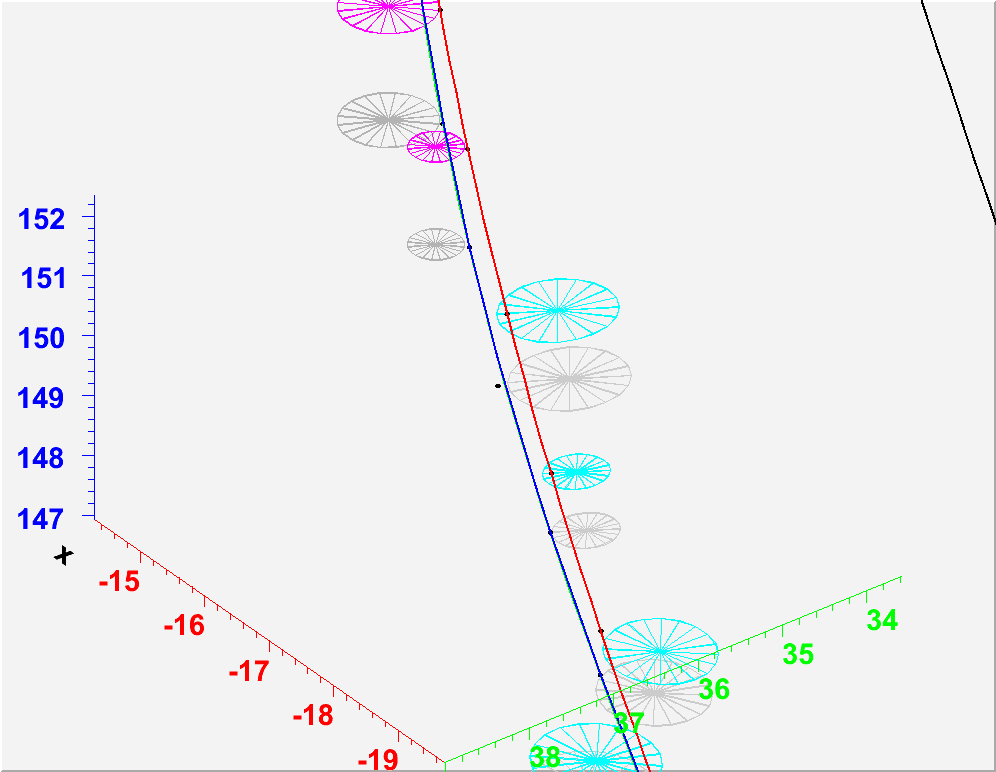
\includegraphics[height=3.0in]{universe.png}
$$
}

\end{document}

\begin{frame}[fragile]
\frametitle{}
\tiny
\begin{verbatim}
\end{verbatim}
\end{frame}
